\documentclass[10pt]{scrreprt}
\usepackage[a4paper, top=30mm, left=25mm, right=25mm, bottom=30mm]{geometry}
\usepackage[utf8]{inputenc}

\usepackage[Bjornstrup]{fncychap}
\usepackage{ngerman}
\usepackage{graphicx}
\usepackage{blindtext,caption}
\usepackage{epstopdf}
\usepackage{etoolbox}
\usepackage{enumitem}
\usepackage{url}
\usepackage{numprint}
\usepackage{longtable}
\usepackage{tabu}
\usepackage{multirow}
\usepackage{caption}
\usepackage{array}
\usepackage{amssymb}
\usepackage{color}
\usepackage{colortbl}
\usepackage{subfigure}
\usepackage{makeidx}
\makeindex



\makeatletter
\patchcmd{\@makechapterhead}{\vspace*{50\p@}}{\vspace*{-20\p@}}{}{}
\patchcmd{\@makeschapterhead}{\vspace*{50\p@}}{\vspace*{7\p@}}{}{}
\patchcmd{\DOTIS}{\vskip 40\p@}{\vskip -12\p@} 
\makeatother
  
\captionsetup[figure]{labelfont={sf,bf},textfont={sf}}
\deffootnotemark{[\thefootnotemark]}
\deffootnote{1.5em}{1em}{[\thefootnotemark] }
\setlength{\parindent}{0pt}
\renewcommand{\labelitemi}{ \raisebox{0.3ex}{\small$\blacktriangleright$} }
\renewcommand{\labelitemii}{ \raisebox{0.3ex}{\small$\triangleright$} }

\newcommand{\sfbf}[1]{\textbf{\sffamily #1}}
\newcommand{\sfit}[1]{\textit{\sffamily #1}}
\newcommand{\W}{\sfbf{W}}
\newcommand{\ziellabel}{Z}
\newcommand{\JoglEarth}{\raisebox{-1.2mm}{
\includegraphics[scale=0.33]{Logo-Text.eps}} }
\newcommand{\textref}[1]{\mbox{\raisebox{0.1ex}{\small$\rightarrow$ }\textit{#1}}}

\newenvironment{details}[1][6pt]{%
  \parskip#1 \parindent6mm \raggedright%
  \def\item{\par\ignorespaces\hangindent=5mm \hangafter1}}{%
  \par\ignorespaces} 

\definecolor{Gray}{gray}{0.9}

\begin{document}

\thispagestyle{empty}
\sffamily
 
\title{Handbuch}

\begin{figure}
\begin{flushright}
	
\includegraphics[scale=0.4]{uniLogo.eps}
\vspace{2.0 cm}
\end{flushright}
\end{figure}

\begin{center}
\vspace{2.0 cm}
{\LARGE SEP – Wintersemester 2013/14}

\vspace{1.0 cm}
\textbf{{\Huge Handbuch}}

\vspace{0.4 cm}
\begin{figure}[!htb]
\begin{center}
	
\includegraphics[scale=1.5]{Logo-Print.eps}
\end{center}
\end{figure}

\vspace{0.2 cm}
\textbf{{\huge OpenStreetMap: Die Welt in 3D}}

\vspace{1.5 cm}
31.01.2014

\vspace{0.5 cm}
Version: 1.0

\vspace{1.5 cm}
{\Large Projektbetreuer: Peter Barth}

\end{center}


\pagebreak
\rmfamily
\tableofcontents


\chapter{Vorwort}
\section*{Ziel \& Zweck}
Dieses Handbuch soll Ihnen als umfassendes Nachschlagewerk zur Bedienung von \JoglEarth dienen. 

\vspace{3mm}
Die ausführlichen Beschreibungen der Abläufe inklusive der Übungsaufgaben sollen das Arbeiten mit der vorliegenden Software erleichtern. 

\vspace{3mm}
\section*{Übungsaufgaben}
Das Lösen der Übungen soll Ihnen die Möglichkeit bieten, die Bedienung von \JoglEarth zu verinnerlichen.

\vspace{3mm}
\section*{Tipps \& Tricks}
Sie erhalten verschiedenste Tipps \& Tricks - die mittels spezieller Symbole gekennzeichnet sind - um effizient mit der Anwendung arbeiten zu können, wie im nachfolgenden Kapitel \textit{\textref Zur Benutzung dieses Handbuchs} beschrieben.

\vspace{3mm}
\section*{Entwicklerteam}
Das Entwicklerteam bestehend aus
\begin{itemize}
\item Christof Blauberger
\item Thomas Eder
\item Gabriele Haas
\item Fabian Knorr
\item Sebastian Reichl
\item Constantin Wenger
\end{itemize}
hat hoffentlich Ihre Neugierde für 'die Welt in 3D' geweckt.\\
Viel Spaß bei der Nutzung von \JoglEarth. 



\chapter{Zur Benutzung dieses Handbuchs}
Im vorliegenden Handbuch werden wichtige Begriffe hervorgehoben.\\

\vspace{5mm}
Die folgende Formatierungen sind im Handbuch zu finden:

\begin{center}
\begin{tabular}{|>{\centering \arraybackslash}m{3cm}|m{10cm}|}
\hline 
\rule[-1ex]{0pt}{3ex} \parbox[0pt][0.5cm][c]{0cm}{} \textbf{Formatierung} & \textbf{Erläuterung} \\
\hline
\hline
\rule[-1ex]{0pt}{4ex} \parbox[0pt][0.9cm][c]{0cm}{} \textbf{fett} & wichtige Schlagwörter, verwendete Begriffe in \JoglEarth \\
\hline
\rule[-1ex]{0pt}{4ex} \parbox[0pt][0.9cm][c]{0cm}{} \textit{kursiv} & kursiv formatierte Texte dienen als Beispiele \\
\hline
\rule[-1ex]{0pt}{4ex} \parbox[0pt][0.9cm][c]{0cm}{} \underline{unterstrichen} & unterstrichene Texte sind zum Üben gedacht, diese Texte stellen Eingaben in \JoglEarth dar \\
\hline
\end{tabular}
\end{center}


\vspace{5mm}
Es werden im Handbuch einige Symbole verwendet, welche die Arbeit mit dem Handbuch erleichtern sollen:

\begin{center}
\begin{tabular}{|>{\centering \arraybackslash}m{3cm}|m{10cm}|}
\hline 
\rule[-1ex]{0pt}{3ex} \parbox[0pt][0.5cm][c]{0cm}{} \textbf{Symbol} & \textbf{Erläuterung} \\ 
\hline
\hline
\rule[-1ex]{0pt}{6ex}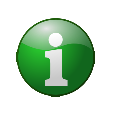
\includegraphics[scale=0.5]{images/info.eps} & Tipps \& Tricks  \\ 
\hline
\rule[-1ex]{0pt}{6ex}
\includegraphics[scale=0.5]{images/quest.eps} & Übungen \\
\hline
\rule[-1ex]{0pt}{3ex} \parbox[0pt][0.9cm][c]{0cm}{} \textref{Kap.} & Hinweis auf ein weiterführendes Kapitel im Handbuch \\
\hline
\end{tabular}
\end{center}

\vspace{5mm}
\begin{tabular}{>{\centering \arraybackslash}m{1cm} m{14cm}}
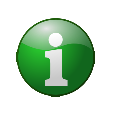
\includegraphics[scale=0.5]{images/info.eps} & \textit{Kursive Textausschnitte} nicht mit der Formatierung für die \textref{weiterführenden Kapitel} verwechseln. 
\end{tabular}

\vspace{5mm}
Die Abbildungen im Handbuch können vom \JoglEarth Erscheinungsbild auf Ihrem PC abweichen, was durch das jeweils verwendete Betriebssystem bedingt ist. Die Funktionalitäten und Anordnungen der Schaltflächen sind jedoch unter allen Betriebssystemen identisch. Die in diesem Handbuch abgebildeten Screenshots wurden teilweise unter Windows und teilweise unter Linux erstellt.\\

\vspace{5mm}
Flussdiagramme erläutern



\chapter{Allgemeines}
\section{Ausgangssituation}
Die Karten des OpenStreetMap-Projekts erfreuen sich immer größerer Beliebtheit. Der Detailgrad, die Menge an verschiedenen Merkmalen und die Genauigkeit der Daten sind denen ihrer Konkurrenz in den meisten Regionen der Welt weit voraus. Durch die große Auswahl an Informationen und die Flexibilität in der Darstellung eröffnen sich unzählige Anwendungsmöglichkeiten.

\vspace{0.5cm}
Die Projektion einer Straßenkarte auf einen dreidimensionalen Globus ist die intuitivste und geographisch korrekteste Darstellung. Bei \JoglEarth wurden folgende Schwerpunkte gesetzt:
\begin{itemize}
\item Verwendung der freien Kartendaten des OpenStreetMap-Projekts
\item Realisierung einer dreidimensionalen Globusoberfläche mit den Höhendaten der NASA \index{NASA}
\item Intuitive Bedienung der Anwendung ohne Einarbeitungszeit
\item Die Möglichkeit der spielerischen Benutzung durch Kinder ohne nennenswerte PC-Kenntnisse
\item Vollständige Plattformunabhängigkeit durch Java
\item Effiziente Speicher- und Bandbreitennutzung
\end{itemize}


\vspace{2mm}
\section{Anwendungsbereich}
\JoglEarth bietet eine dreidimensionale Ansicht der Welt sowie eine ebene Kartenansicht. Beides erfolgt auf Basis des OpenStreetMap-Projekts und den Satellitendaten der NASA. \\

Die grafische Benutzeroberfläche zeigt dafür im dreidimensionalen Modus eine Weltkugel, die frei gedreht und gezoomt werden kann und im zweidimensionalen einen Ausschnitt der Weltkarte. Die Karte kann aus verschiedenen Kategorien wie Satellitenbildern oder Straßenkarten gewählt werden. Die Steuerung erfolgt mit Tastatur und Maus. \\

Mit einer Suchfunktion \index{Suche} kann im Umkreis oder global nach Orten gesucht werden. Punkte besonderen Interesses wie Gaststätten oder Banken können über dem Kartenbild eingeblendet werden.


\vspace{3mm}
\section{Zielgruppe}
Primäre Zielgruppe des Systems sind Privatanwender, die eine andere Art der Kartendarstellung als die der typischen Onlinekarten bevorzugen. \\

Auch soll die Anwendung wissbegierige Kinder ansprechen. Voraussetzung ist lediglich der geübte Umgang mit der Maus und/ oder Tastatur.


\vspace{3mm}
\section{Sicherheit, Datenschutz}
\JoglEarth wahrt von vornherein die Sicherheit des Systems und schützt die Privatsphäre des Nutzers. Da sie keine sicherheitskritischen Daten verarbeitet. 
\begin{itemize}
\item Es ist weder zur Bedienung, noch zum Beschaffen der Kartendaten eine Authentifikation erforderlich.
\item Es werden keine persönlichen Daten des Anwenders über das Netz übertragen.
\item Es wird kein Code aus dem Netz nachgeladen und ausgeführt.
\item Das Programm hat keine (unter Umständen angreifbare) Serverfunktionalität.
\end{itemize}

\vspace{3mm}
\section{Lizenzen}
Lizenzen der verwendeten Bibliotheken und Datenquellen:
\begin{itemize}
\item Die Teile der JOGL-Bibliothek sind unter mehreren Versionen der BSD-Lizenz, der SGI Free Software License und der Apache-Lizenz, der Ubuntu Font License und mehreren proprietären Lizenzen veröffentlicht. Details dazu finden sich bei  \footnote{\url{https://jogamp.org/git/?p=jogl.git;a=blob;f=LICENSE.txt}}.
\item OpenStreetMap ist „OpenData“ im Sinne der Open Database Lizenz (ODbL). Die Kartenkacheln stehen unter der Lizenz  Creative Commons „Namensnennung, Weitergabe unter gleichen Bedingungen" 2.0 (CC BY-SA). Weitere Infos, wie auch eine Vorgabe zum Hinweisen auf die Urheberschaft des OSM-Projekts finden sich bei \footnote{\url{http://www.openstretmap.org/copyright}}.
\item Die Daten der Overpass API sowie Nominatim stehen ebenfalls unter der ODbL.
\item Die Satellitenbilder der NASA sind für die Zwecke des Projekts frei verfügbar und stehen unter der Lizenz, die sich bei \footnote{\url{http://www.nasa.gov/audience/formedia/features/MP_Photo_Guidelines.html}} findet.
\item Die Verwendete Bibliothek JGoodies Forms steht unter der BSD-Lizenz bei \footnote{\url{http://opensource.org/licenses/bsd-license.html}}.
\end{itemize}




\chapter{Systemvoraussetzungen} \index{Systemvoraussetzungen}
\section{Software}
Da das Projekt auf Java setzt, ist es betriebssystemunabhängig. Es muss lediglich das Java Runtime Environment (JRE) in Version 7 sowie ein Fenstersystem und Netzwerkunterstützung zur Verfügung stehen. Um dieses Handbuch anzeigen zu können, muss auf dem System außerdem ein PDF-Betrachter installiert sein. Zusätzliche Programmbibliotheken, die zum Ausführen des Softwarepakets nötig sind, wurden mitgeliefert.\\

Folgende Konfigurationen sollen mindestens unterstützt werden:
\begin{itemize}
\item Windows 7 und 8 auf x86{\_}64 mit den Herstellertreibern von nVidia und AMD
\item Linux auf x86{\_}64 mit X.org und proprietären Treibern von nVidia / AMD sowie den freien radeon-Treibern für AMD
\end{itemize}

\vspace{3mm}
\section{Hardware}
Wie schon bei der Software der Fall sollte die Anwendung auch mit nahezu allen modernen Desktopsystemen kompatibel sein. Folgende (oder eine gleichwertige) Konfiguration wird jedoch für ein optimales Benutzererlebnis mindestens empfohlen:
\begin{itemize}
\item Dual-Core-Prozessor mit 1 GHz Taktfrequenz
\item 2 Gigabyte RAM
\item 200 Megabyte freier Speicherplatz
\item Grafikkarte: Onboard-Grafik mit OpenGL 2.0-Unterstützung
\item Bildschirm mit 1024x768 Pixeln Auflösung und 24 Bit Farbtiefe
\item Standard-Tastatur und Maus
\end{itemize}

\vspace{3mm}
\section{Orgware}
Zum Laden der Kartendaten wird eine durchgehende Internetverbindung benötigt. Um die Wartezeiten akzeptabel zu halten wird mindestens 1MBit/s empfohlen.





\chapter{Erste Schritte}


\section{Starten von JoglEarth}
Öffnen von \textbf{joglearth.jar} durch Doppelklick auf die Datei.\\
\JoglEarth startet in der folgenden \textref{Benutzeroberfläche}:

\vspace{3mm}
\begin{center}
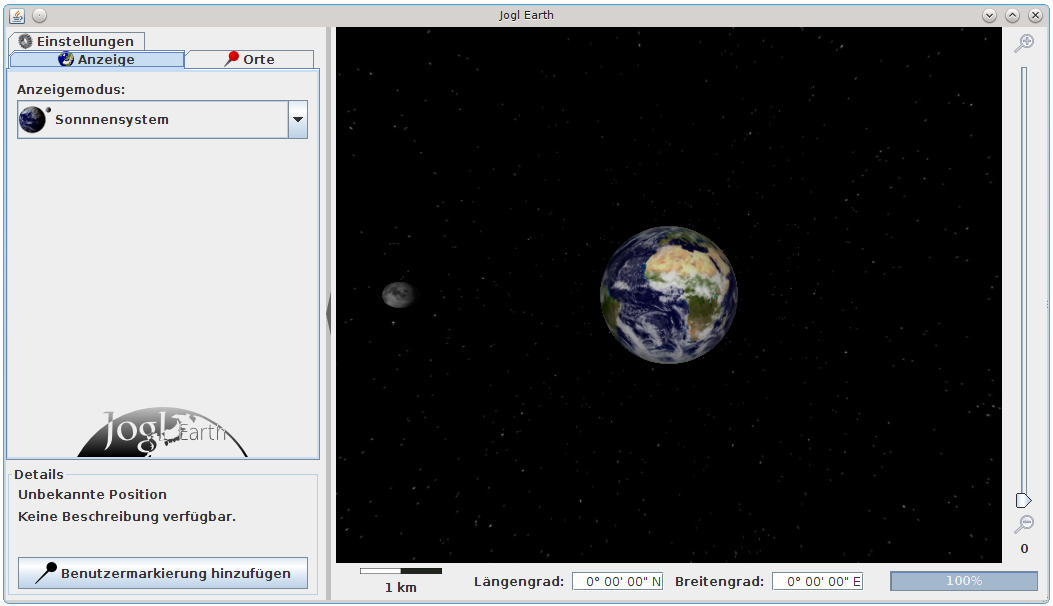
\includegraphics[scale=0.4]{images/sonnensystem.png}
\end{center}

\vspace{5mm} \index{Sonnensystem}
\begin{tabular}{>{\centering \arraybackslash}m{1cm} m{14cm}}
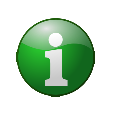
\includegraphics[scale=0.5]{images/info.eps} & \JoglEarth startet standardmäßig in der \textbf{Sonnensystemansicht} (\textref{Ansichtsmodi}).
\end{tabular}

\vspace{3mm} \index{Sonnensystem}
\begin{tabular}{>{\centering \arraybackslash}m{1cm} m{14cm}}
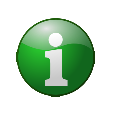
\includegraphics[scale=0.5]{images/info.eps} & Die \textbf{Sprache} der Benutzeroberfläche kann im \textref{Menü Einstellungen} festgelegt werden. Die Vorgehensweise hierzu findet sich im Kapitel \textref{Sprache}.
\end{tabular}

\vspace{3mm}
\begin{tabular}{>{\centering \arraybackslash}m{1cm} m{14cm}}

\includegraphics[scale=0.5]{images/quest.eps} &  Versuchen Sie nun \JoglEarth zu starten. Machen Sie sich mit der Benutzeroberfläche vertraut.
\end{tabular}

\vspace{5mm} \index{Benutzeroberfläche} \index{Navigation Globus / Kartenebene}
In den folgenden Kapiteln finden Sie als Einführung die Erklärungen zur \textref{Benutzeroberfläche}, zur \textref{Navigation} auf dem Globus und der Kartenebene.


\newpage
\section{Benutzeroberfläche} \index{Benutzeroberfläche} \index{Benutzeroberfläche!Ansichtsfenster} \index{Ansichtsfenster} \index{Benutzeroberfläche!Seitenleiste} \index{Seitenleiste} \index{Benutzeroberfläche!Statusleiste} \index{Statusleiste}
\vspace{3mm}
\subsection{Bildschirmaufbau / Fensteransichten}
\begin{itemize}
	\item Das Hauptelement der Benutzeroberfläche ist das \textbf{Ansichtsfenster}  \raisebox{-1pt}{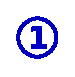
\includegraphics[scale=0.45]{images/1.eps}}, das sich in der Fenstermitte befindet. Darin wird der Globus, die Kartenebene oder eine Sonnensystemansicht angezeigt. Der sichtbare Kartenausschnitt kann interaktiv mit Maus oder Tastatur verschoben, gedreht gezoomt und gekippt werden.
	\item Am linken Rand des Fensters befindet sich die \textbf{Seitenleiste} \raisebox{-1pt}{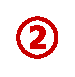
\includegraphics[scale=0.45]{images/2.eps}}, die die meisten Steuerungsoptionen bereitstellt. Der obere Teil ist in Menüs unterteilt, mit denen Funktionen gruppiert werden; der untere Teil zeigt Details zum momentan zentrierten Punkt an. Um den sichtbaren Kartenbereich zu vergrößern, ist sie ausblendbar.
	\item Am rechten Rand \raisebox{-1pt}{
\includegraphics[scale=0.45]{images/3.eps}} befindet sich ein Schieber, mit dem das Zoomlevel angezeigt und geändert werden kann.
	\item Die \textbf{Statusleiste} \raisebox{-1pt}{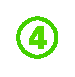
\includegraphics[scale=0.45]{images/4.eps}} am unteren Rand beinhaltet Informationen über den zentrierten Punkt, wie Koordinaten und Maßstab. Außerdem wird der Fortschritt im Hintergrund geladener Daten angezeigt.
\end{itemize}

\vspace{3mm}
\begin{center}
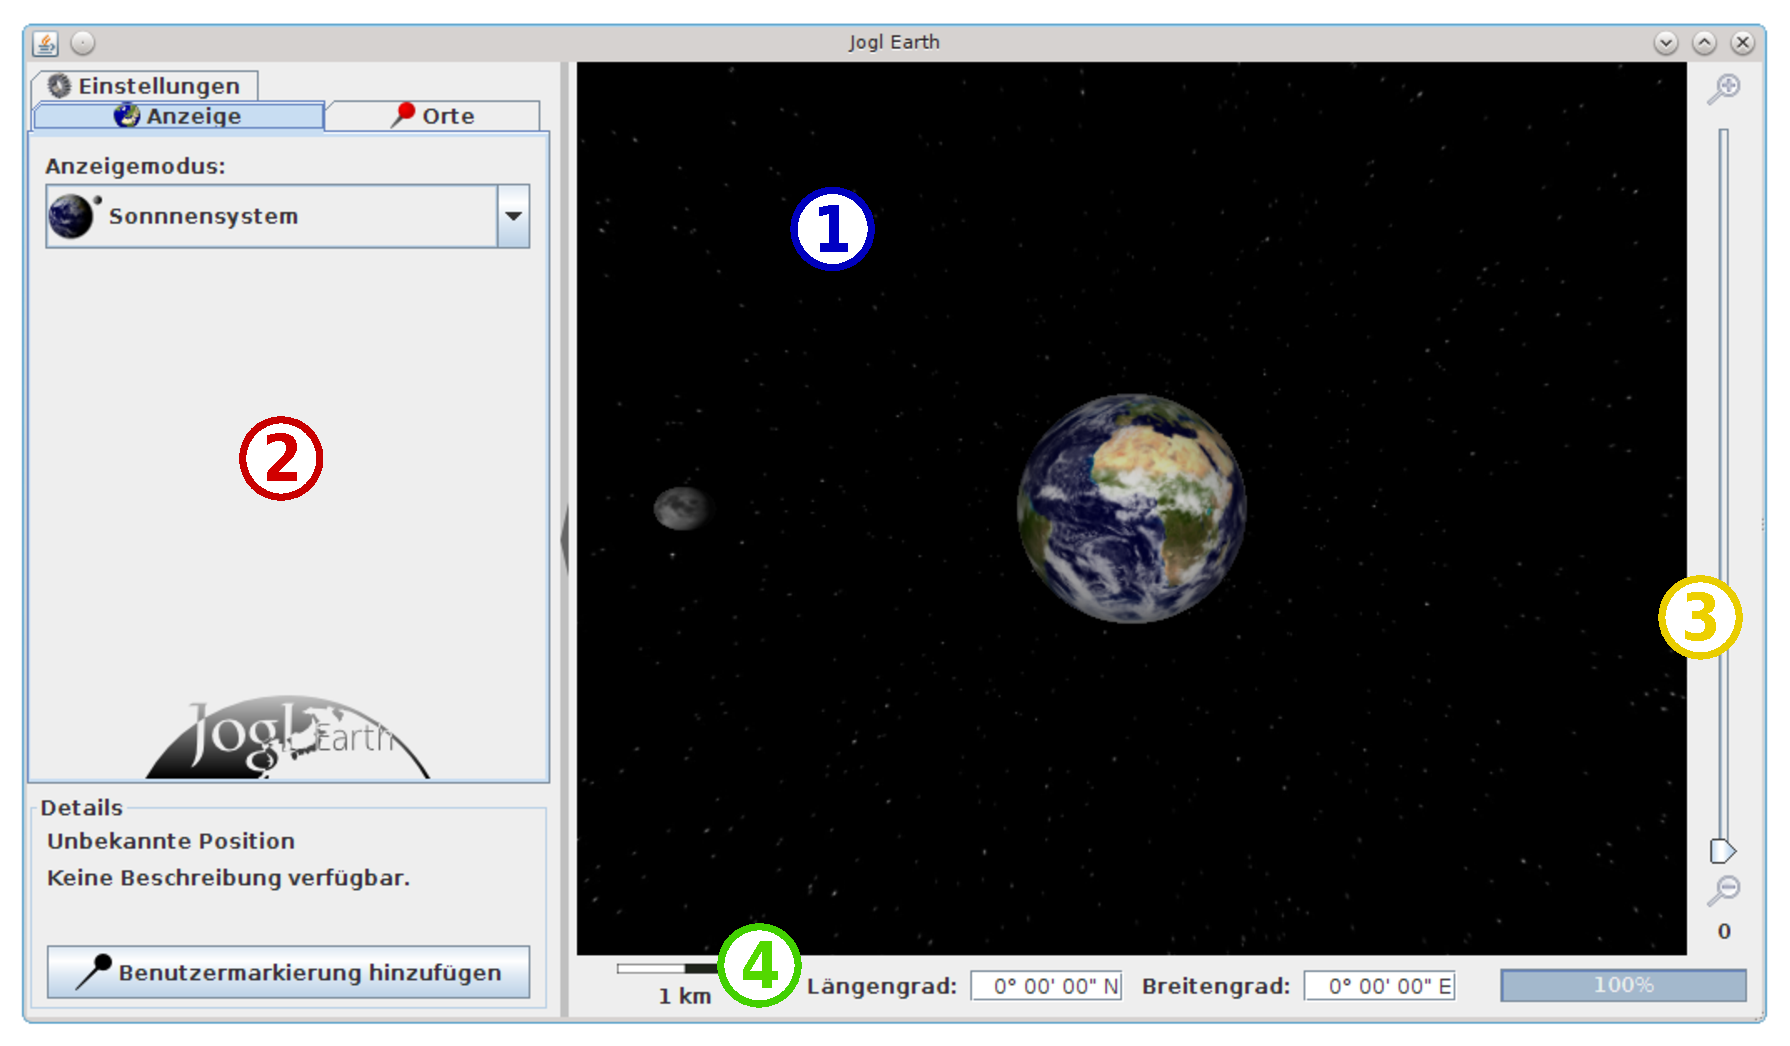
\includegraphics[scale=0.5]{images/uebersicht.eps}
\end{center}

\newpage
\subsection{Menüführung} \index{Menüführung} \index{Benutzeroberfläche!Seitenleiste} \index{Seitenleiste}
Die gesamte Menüführung befindet sich in der linken \textbf{Seitenleiste} und gruppiert die wichtigsten Funktionalitäten (\textref{Funktionen}) von \JoglEarth . 

\vspace{3mm}
\begin{tabular}{>{\centering \arraybackslash}m{1cm} m{14cm}} \index{Menüführung!Menü Details} \index{Menü Details}
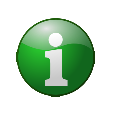
\includegraphics[scale=0.5]{images/info.eps} & Der Bereich \textbf{Details} in den angeführten Menüs verändert sich beim Wechseln der Menüs nicht.
\end{tabular}

\vspace{3mm}
\begin{tabular}{>{\centering \arraybackslash}m{1cm} m{14cm}} \index{Benutzeroberfläche!Seitenleiste} \index{Seitenleiste}
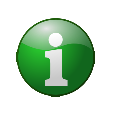
\includegraphics[scale=0.5]{images/info.eps} & Sollte die \textbf{Seitenleiste} nicht sichtbar sein, ist diese möglicherweise ausgeblendet.
\end{tabular}

\vspace{3mm}
\begin{tabular}{>{\centering \arraybackslash}m{1cm} m{14cm}} \index{Benutzeroberfläche!Seitenleiste} \index{Seitenleiste}

\includegraphics[scale=0.5]{images/quest.eps} & Blenden Sie die \textbf{Seitenleiste} aus und anschließend wieder ein.
\end{tabular}


\vspace{10mm}
\begin{minipage}[t]{9cm}
\vspace{-40mm}
\subsubsection{1. Menü: Ansicht} \index{Menü Ansicht} \index{Menüführung!Menü Ansicht}
	\begin{itemize}
	\item Ändern der \textref{Ansichtsmodi} \index{Ansichtsmodi}
	\item Ändern der \textref{Kartentypen} \index{Kartentypen}
	\item \textref{Höhenprofil} zu- oder abschalten \index{Höhenprofil}
	\end{itemize}
\end{minipage}
\begin{minipage}{7cm}
\centering
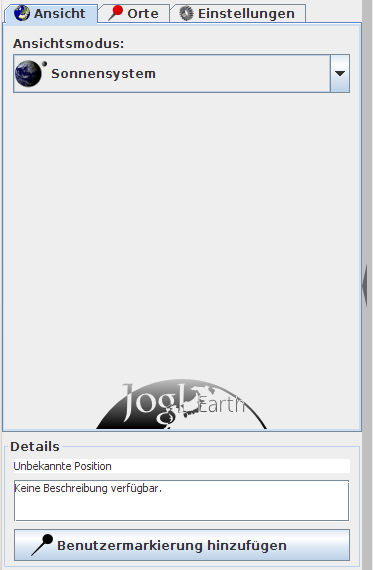
\includegraphics[scale=0.4]{images/anzeige_tab.png}
\end{minipage}



\vspace{10mm}
\begin{minipage}[t]{9cm}
\vspace{-40mm}
\subsubsection{2. Menü: Orte} \index{Menü Orte} \index{Menüführung!Menü Orte}
	\begin{itemize}
	\item \textref{Suche} nach gewünschten Orten \index{Suche}
	\item Anzeige der Suchergebnisse
	\item Anzeige der gespeicherten \textref{Benutzermarkierungen} \index{Benutzermarkierungen}
	\item Ein- und ausblenden diverser \textref{Overlays} \index{Overlays}
	\end{itemize}
\end{minipage}
\begin{minipage}{7cm}
\centering
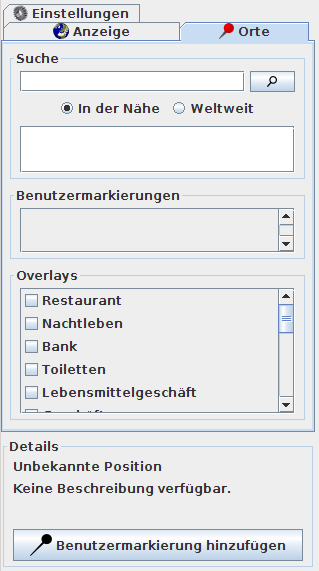
\includegraphics[scale=0.4]{images/orte_tab.png}
\end{minipage}




\newpage
\begin{minipage}[t]{9cm}
\vspace{-40mm}
\subsubsection{3. Menü: Einstellungen} \index{Menü Einstellungen} \index{Menüführung!Menü Einstellungen}
	\begin{itemize}
	\item Ändern der \textref{Sprache} \index{Sprache} \index{Benutzeroberfläche!Sprache}
	\item Ändern von \textref{Grafikeinstellungen} \index{Grafikeinstellungen}
	\item Festlegen der \textref{Cachegrößen} \index{Cachegrößen}
	\item Anzeige des Handbuchs im PDF-Format
	\item Anzeige des 'Über-uns-Fensters'
	\end{itemize}
\end{minipage}
\begin{minipage}{7cm}
\centering
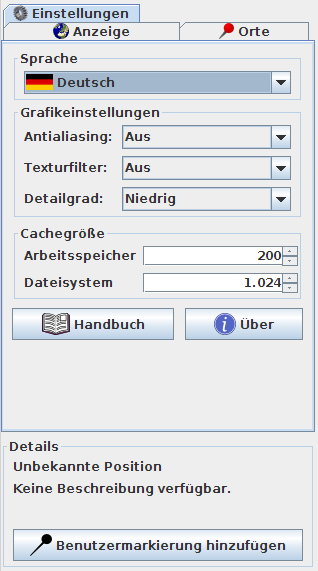
\includegraphics[scale=0.4]{images/einstellungen_tab_DE.png}
\end{minipage}


\vspace{5mm}
\subsubsection{4. Menü: Details} \index{Menü Details} \index{Benutzermarkierungen} \index{Menüführung!Menü Details}

\begin{itemize}
\item Erstellen von \textref{Benutzermarkierungen}
\end{itemize}


\vspace{3mm}
\begin{tabular}{>{\centering \arraybackslash}m{1cm} m{14cm}} \index{Menüführung!Menü Details} \index{Menü Details}
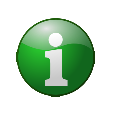
\includegraphics[scale=0.5]{images/info.eps} & Der Bereich \textbf{Details} in den angeführten Menüs verändert sich beim Wechseln der Menüs nicht.
\end{tabular}

\vspace{5mm}
\begin{minipage}[t]{9cm}
\vspace{-10mm}
Der Bereich \textbf{Details} zeigt verfügbare Informationen genau zum Bildmittelpunkt des aktuellen Kartenausschnitts an. Der Bildmittelpunkt ist mit einem Rautensymbol gekennzeichnet. Ebenso findet sich hier die Schaltfläche um \textref{Benutzermarkierungen} zu setzen und wieder zu entfernen. \\
\end{minipage}
\begin{minipage}{7cm}
\centering
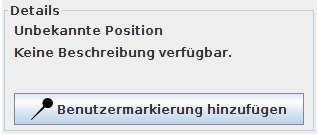
\includegraphics[scale=0.4]{images/details_menu.png}
\end{minipage}

\vspace{3mm}
Beispiel:
\begin{itemize}
\item \textit{Angenommen im Bildmittelpunkt des Kartenausschnitts befindet sich das Finanzamt der Stadt Regensburg, dann wird im Bereich \textbf{Details} 'Finanzamt Regensburg' angezeigt.}
\end{itemize}

\vspace{3mm}
\begin{tabular}{>{\centering \arraybackslash}m{1cm} m{14cm}}
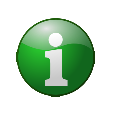
\includegraphics[scale=0.5]{images/info.eps} & Informationen zum Bildmittelpunkt des aktuellen Kartenausschnitts werden erst ab hohen Zoomstufen verfügbar.
\end{tabular}




\newpage
\subsection{Navigation der Erde / Kartenebene} \index{Navigation Globus / Kartenebene}

\vspace{3mm}
\subsubsection*{Mausbelegung} \index{Navigation Globus / Kartenebene!Mausbelegung}
\begin{tabular}{|>{\centering \arraybackslash}m{3cm}|m{10cm}|}
\hline
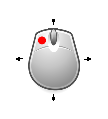
\includegraphics[scale=1.0]{images/mouseDrag_left.eps} & Drehen der Erdkugel / Verschieben der Karte \\ 
\hline 

\includegraphics[scale=1.0]{images/mouseDoubleClick_left.eps} & Punkt unter dem Mauszeiger im Kartenfenster zentrieren \\
\hline
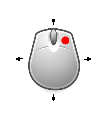
\includegraphics[scale=1.0]{images/mouseDrag_right.eps} & Kippen der Ansicht \\
\hline
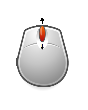
\includegraphics[scale=1.0]{images/mouse_scrollen.eps} & Zoomen der Ansicht \\
\hline
\end{tabular} 


\vspace{3mm}
\subsubsection*{Tastaturbelegung} \index{Navigation Globus / Kartenebene!Tastaturbelegung}
\begin{tabular}{|>{\centering \arraybackslash}m{3cm}|m{10cm}|}
\hline
\rule[-1ex]{0pt}{7ex}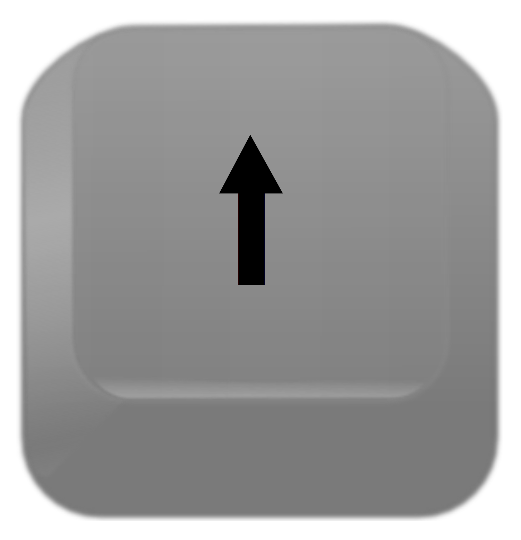
\includegraphics[scale=0.08]{images/key_arrow_up.eps}& \multirow{3}{*}{Drehen der Erdkugel / Verschieben der Karte}\\
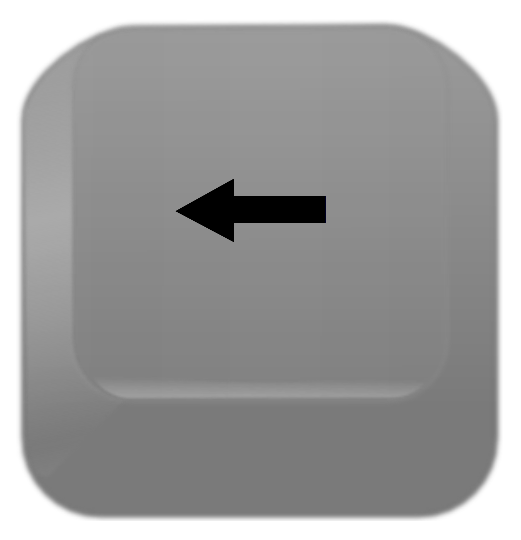
\includegraphics[scale=0.08] {images/key_arrow_left.eps} 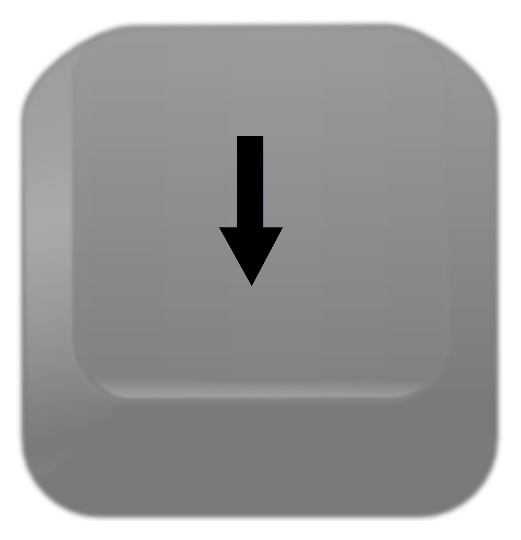
\includegraphics[scale=0.08]{images/key_arrow_down.eps} 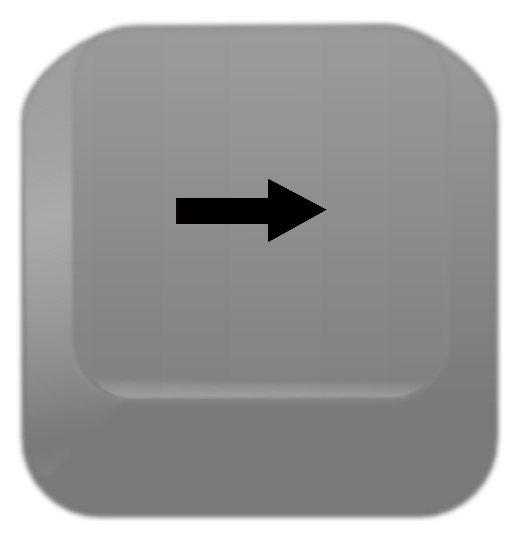
\includegraphics[scale=0.08]{images/key_arrow_right.eps} &  \\
\hline
\rule[-1ex]{0pt}{7ex} 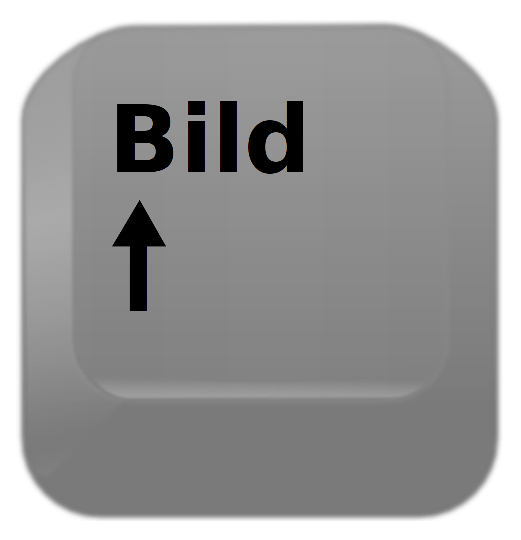
\includegraphics[scale=0.08]{images/key_Bild_Auf.eps}  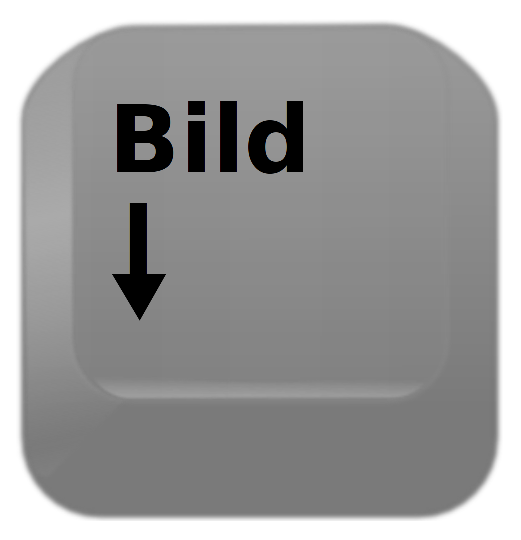
\includegraphics[scale=0.08]{images/key_Bild_Ab.eps} & Kippen der Ansicht nach oben / unten\\
\hline
\rule[-1ex]{0pt}{7ex} 
\includegraphics[scale=0.08]{images/key_Pos1.eps} 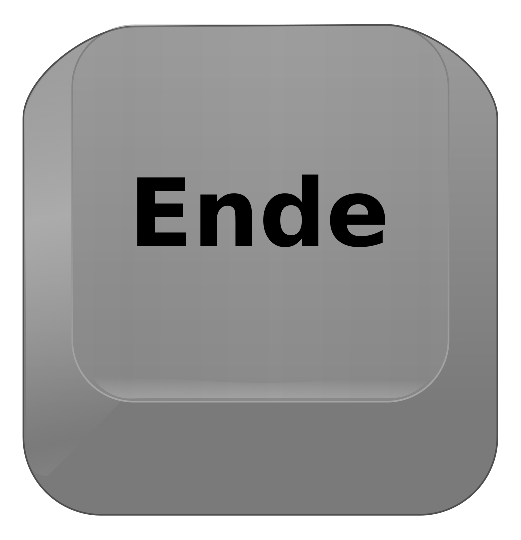
\includegraphics[scale=0.08]{images/key_Ende.eps} & Kippen der Ansicht nach links / rechts \\
\hline
\rule[-1ex]{0pt}{7ex} 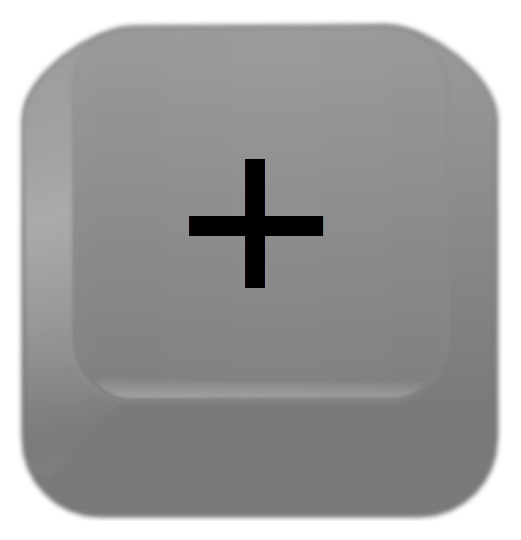
\includegraphics[scale=0.08]{images/key_Plus.eps}  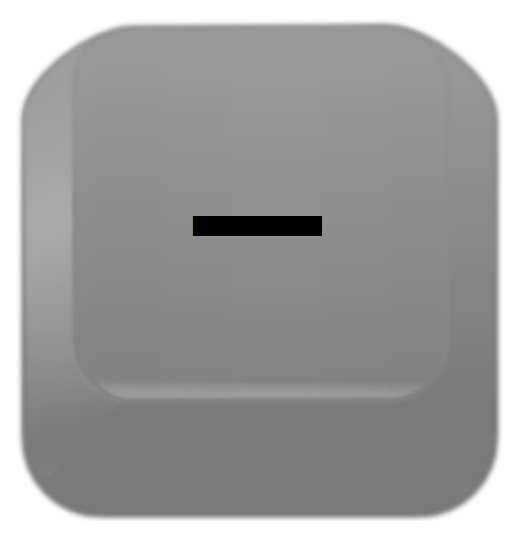
\includegraphics[scale=0.08]{images/key_Minus.eps} & Zoomen der Ansicht \\
\hline
\rule[-1ex]{0pt}{7ex} 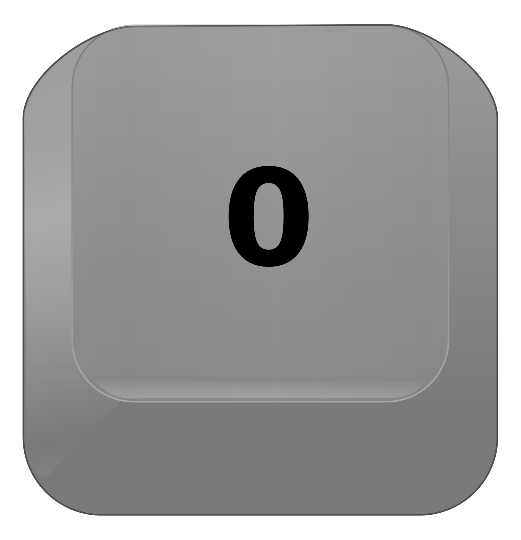
\includegraphics[scale=0.08]{images/key_0.eps} & Rücksetzen des Kippens \\ 
\hline
\rule[-1ex]{0pt}{7ex} 
\includegraphics[scale=0.08]{images/key_F1.eps} & Anzeige des Benutzerhandbuchs \\ 
\hline
\rule[-1ex]{0pt}{7ex} 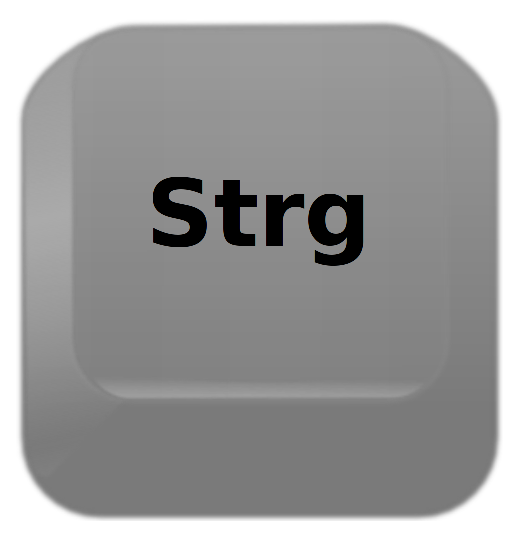
\includegraphics[scale=0.08]{images/key_Strg.eps} \rule[-1ex]{0pt}{7ex}\raisebox{0.7em}{\textbf{+}} 
\includegraphics[scale=0.08]{images/key_Q.eps} & Beenden der Anwendung \\ 
\hline
\end{tabular}


\newpage
\section{Standard-Einstellungen}
Bei erstmaligem Starten von \JoglEarth sind standardmäßig folgende Einstellungen gesetzt:

\begin{itemize}
\item Ansichtsmodus: Sonnensystem
\item Kartentyp: -
\item Höhenprofil: deaktiviert
\item Zoomlevel: 0\%
\item Overlays: alle deaktiviert
\item Sprache: Deutsch
\item Grafikeinstellungen:
	\begin{itemize}
	\item Antialiasing: deaktiviert
	\item Textur Filter: Nächster Nachbar
	\item Detailgrad: niedrig
	\end{itemize}
\item Cachegrößen [MB]:
	\begin{itemize}
	\item Arbeitsspeicher: 200
	\item Dateisystem: 1.000
	\end{itemize}
\end{itemize}



\chapter{Ansichtsmodi} \index{Ansichtsmodi}
\JoglEarth bietet zahlreiche Darstellungsmöglichkeiten für diverse Ansichten. Im folgenden werden die wählbaren Modi kurz erklärt.

\vspace{3mm}
\section{Sonnensystem} \index{Ansichtsmodi!Sonnensystem} \index{Sonnensystem}
Diese Ansicht stellt ein detailliertes Modell von Sonne, Mond und Erde dar, wobei der Mond um die Erde kreist.

\vspace{3mm}
\begin{tabular}{>{\centering \arraybackslash}m{1cm} m{14cm}}
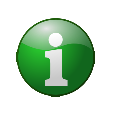
\includegraphics[scale=0.5]{images/info.eps} &  Navigation: Das Sonnensystem kann gedreht und gekippt werden.
\end{tabular}

\vspace{3mm}
\begin{tabular}{>{\centering \arraybackslash}m{1cm} m{14cm}}
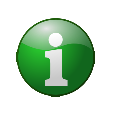
\includegraphics[scale=0.5]{images/info.eps} &  Funktionalität: In dieser Ansicht können keine weiteren Funktionalitäten genutzt werden, wie beispielsweise \textref{Ändern von Längen- und Breitengraden}, \textref{Ändern des Zoomlevels}, Aktivieren des \textref{Höhenprofils}, \textref{Markierungen setzen}.
\end{tabular}

\vspace{3mm}
\begin{center}
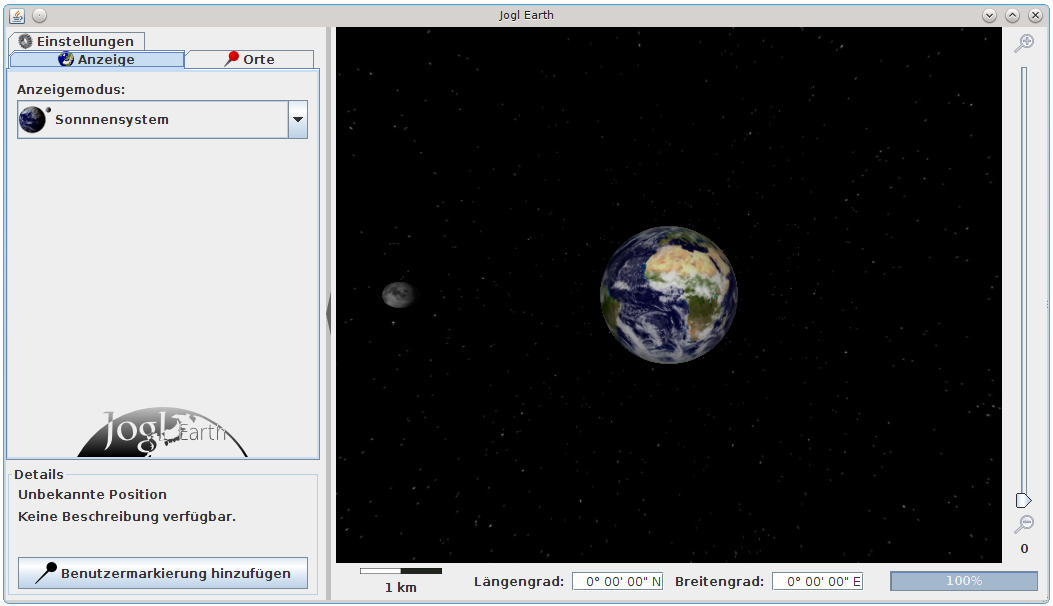
\includegraphics[scale=0.3]{images/sonnensystem.png}
\end{center}



\newpage
\section{Globus} \index{Ansichtsmodi!Globus} \index{Globus} \index{Kartentypen}
Diese Ansicht visualisiert einen Globus, welcher die Anzeige von den verfügbaren \textref{Kartentypen} unterstützt.


\vspace{3mm}
\begin{tabular}{>{\centering \arraybackslash}m{1cm} m{14cm}}
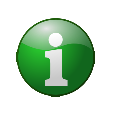
\includegraphics[scale=0.5]{images/info.eps} &  Navigation: Der Globus kann gedreht, vergrößert, verkleinert und gekippt werden.
\end{tabular}

\vspace{3mm}
\begin{tabular}{>{\centering \arraybackslash}m{1cm} m{14cm}}
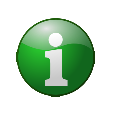
\includegraphics[scale=0.5]{images/info.eps} &  Funktionalität: Diese Ansicht unterstützt die gesamte Funktionalität von \JoglEarth , wie beispielsweise Aktivieren des \textref{Höhenprofils}, \textref{Markierungen setzen}, etc.
\end{tabular}

\vspace{3mm}
\begin{center}
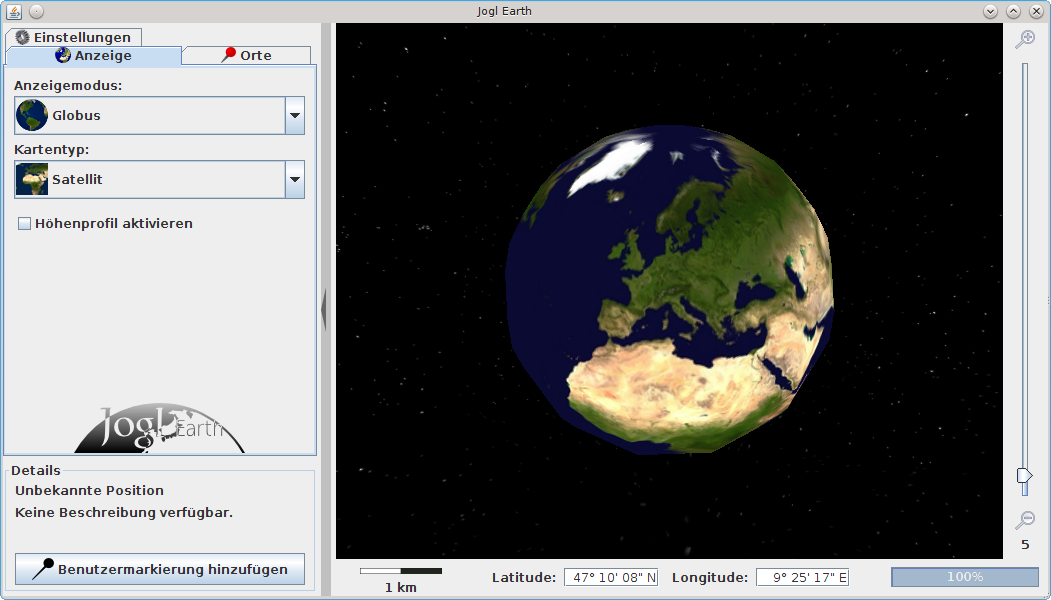
\includegraphics[scale=0.3]{images/globus-satellit.png}
\end{center}




\vspace{3mm}
\section{Kartenebene} \index{Ansichtsmodi!Kartenebene} \index{Kartenebene} \index{Kartentypen}
Diese Ansicht visualisiert eine Kartenebene, welche die Anzeige von den verfügbaren \textref{Kartentypen} unterstützt.


\vspace{3mm}
\begin{tabular}{>{\centering \arraybackslash}m{1cm} m{14cm}}
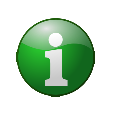
\includegraphics[scale=0.5]{images/info.eps} &  Navigation: Die Kartenebene kann gedreht, vergrößert, verkleinert und gekippt werden.
\end{tabular}

\vspace{3mm}
\begin{tabular}{>{\centering \arraybackslash}m{1cm} m{14cm}}
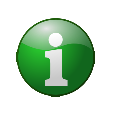
\includegraphics[scale=0.5]{images/info.eps} &  Funktionalität: Diese Ansicht unterstützt die gesamte Funktionalität von \JoglEarth , wie beispielsweise Aktivieren des \textref{Höhenprofils}, \textref{Markierungen setzen}, etc.
\end{tabular}

\vspace{3mm}
\begin{center}
\includegraphics[scale=0.3]{images/flacheKarte_satellit.png}
\end{center}







\chapter{Kartentypen} \index{Kartentypen}
\JoglEarth bietet zahlreiche Kartentypen, die im folgenden näher betrachtet werden.

\vspace{3mm}
\begin{tabular}{>{\centering \arraybackslash}m{1cm} m{14cm}}
\includegraphics[scale=0.5]{images/info.eps} &  Im folgenden wurden alle Abbildungen in der Ansicht \textref{Kartenebene} (\textref{Ansichtsmodi}) gemacht, um die Unterschiede der Kartentypen eindeutig hervorzuheben.
\end{tabular}


\vspace{3mm}
\section{Satellit} \index{Kartentypen!Satellit} \index{Satellit}
Unter diesem Kartentyp versteht man Satellitenbilder, welche Aufnahmen der Erdoberfläche aus der Perspektive eines Satelliten zeigen.

\vspace{3mm}
\begin{center}
\includegraphics[scale=0.3]{images/flacheKarte_satellit.png}
\end{center}



\vspace{3mm}
\section{OpenStreetMap} \index{Kartentypen!OpenStreetMap} \index{OpenStreetMap}
\JoglEarth setzt auf die folgenden freien Kartenmaterialien des OpenStreetMap-Projekts, welche von den jeweiligen Servern zeitnahe geladen werden.


\subsection{Straßenkarte} \index{OpenStreetMap!Straßenkarte} \index{Straßenkarte}
Die \textbf{Straßenkarte} ist eine thematische Karte, die den Schwerpunkt auf den Straßenverlauf und das Straßenverkehrsnetz setzt.


\vspace{3mm}
\begin{figure}[!htb]
	\centering
    \subfigure{\includegraphics[scale=0.2]{images/flacheKarte_Strassenkarte1.png}}
    \hspace{5mm}
% Es fehlen bei der Straßenkarte noch die Labels, deshalb hab ich den zweiten Screenshot noch nicht gemacht.    
%    \subfigure{\includegraphics[scale=0.2]{images/flacheKarte_Strassenkarte2.png}}
\end{figure} 

\vspace{3mm}
\begin{tabular}{>{\centering \arraybackslash}m{1cm} m{14cm}}
\includegraphics[scale=0.5]{images/info.eps} & Das detaillierte Straßenverkehrsnetz wird ab Zoomlevel ?? ersichtlich.
\end{tabular}




\subsection{Radkarte} \index{OpenStreetMap!Radkarte} \index{Radkarte}
Bei der \textbf{Radkarte} (bzw. Radwegkarte, Fahrradkarte) handelt es sich um eine thematische Karte, die speziell auf die Bedürfnisse von Radfahrern zugeschnitten ist. Es werden Radwege mit deren Bezeichnung bzw. Nummerierung angezeigt. Zweck der Radkarte ist es, Wege zu finden, die für Radfahrer freigegeben sind.

\vspace{3mm}
\begin{figure}[!htb]
	\centering
    \subfigure{\includegraphics[scale=0.205]{images/flacheKarte_Radkarte1.png}}
    \hspace{5mm}
    \subfigure{\includegraphics[scale=0.205]{images/flacheKarte_Radkarte2.png}}
\end{figure} 





\subsection{Landkarte} \index{OpenStreetMap!Landkarte} \index{Landkarte}
Die \textbf{Landkarte} ist eine Straßenkarte, in der die Bezeichnungen in der jeweiligen Landessprache und der landestypischen Gestaltung gehalten sind.

\vspace{3mm}
\begin{figure}[!htb]
	\centering
    \subfigure{\includegraphics[scale=0.199]{images/flacheKarte_Landkarte1.png}}
    \hspace{5mm}
    \subfigure{\includegraphics[scale=0.199]{images/flacheKarte_Landkarte2.png}}
\end{figure}




\subsection{Wanderkarte} \index{OpenStreetMap!Wanderkarte} \index{Wanderkarte}
Die \textbf{Wanderkarte} ist eine Karte, die der unmittelbaren Orientierung im Gelände dient. Zweck der Wanderkarte ist es, Wege zu finden, die für Wandertouren freigegeben sind.

\vspace{3mm}
\begin{figure}[!htb]
	\centering
    \subfigure{\includegraphics[scale=0.199]{images/flacheKarte_Wanderkarte1.png}}
    \hspace{5mm}
    \subfigure{\includegraphics[scale=0.199]{images/flacheKarte_Wanderkarte2.png}}
\end{figure} 



\subsection{OSM2World} \index{OpenStreetMap!OSM2World} \index{OSM2World}
Die \textbf{OSM2World-Karte} errechnet auf Basis der OpenStreetMap-Daten 3D Modelle. Derzeit sind nur einige Teile in Deutschland, in Österreich und in der Schweiz erfasst.

% Screenshots


\section{Kinderkarte} \index{Kartentypen!Kinderkarte} \index{Kinderkarte}
Ein besonderer Kartentyp ist die Kinderkarte. Diese zeigt die einzelnen Kontinente, welche farblich unterschiedlich sind und zusätzlich werden beispielhaft je Kontinent, die dort einheimischen Tiere gezeigt. Dieser Kartentyp ist speziell für Kinder gedacht um die Neugierde an geografischen Karten zu wecken.

\vspace{3mm}
\begin{center}
\includegraphics[scale=0.3]{images/flacheKarte_Kinderweltkarte.png}
\end{center}

\vspace{3mm}
\begin{tabular}{>{\centering \arraybackslash}m{1cm} m{14cm}}
\includegraphics[scale=0.5]{images/info.eps} &  Für Kinder: Es kann von der Kinderkarte im Kartentyp \textref{Kartenebene} in \textref{Satellit} gewechselt werden um den Übergang und die Orientierung auf geografische Karten einfach zu gestalten.
\end{tabular}



\vspace{3mm}
\section*{Platzhaltertextur} \index{Platzhaltertextur}
\begin{minipage}[t]{9cm}
\vspace{-20mm}
Die Platzhaltertextur erscheint, solange das Kartenmaterial geladen wird. Sollten Kartenausschnitte nicht verfügbar sein, wird die Platzhaltertextur ebenfalls angezeigt. Diese zeigt ein grau-weißes Schachbrettmuster.
\end{minipage}
\begin{minipage}{7cm}
\centering
\begin{tabular}{p{0.7cm}p{0.7cm}p{0.7cm}p{0.7cm}}
\parbox[0pt][1cm][c]{0cm}{} \cellcolor{Gray} & & \cellcolor{Gray} &  \\ 
\parbox[0pt][1cm][c]{0cm}{} & \cellcolor{Gray} & & \cellcolor{Gray}\\ 
\parbox[0pt][1cm][c]{0cm}{} \cellcolor{Gray} & & \cellcolor{Gray} &  \\ 
\parbox[0pt][1cm][c]{0cm}{} & \cellcolor{Gray} & & \cellcolor{Gray}\\ 
\end{tabular}
\end{minipage}



\vspace{8mm}
\begin{tabular}{>{\centering \arraybackslash}m{1cm} m{14cm}}
\includegraphics[scale=0.5]{images/quest.eps} &  Versuchen Sie sich durch die zahlreichen Ansichten und Kartentypen zu navigieren.
\end{tabular}









\chapter{Funktionen}
\JoglEarth bietet zahlreiche Funktionen und Optionen, die im folgenden näher betrachtet werden.

\vspace{3mm}
\begin{tabular}{>{\centering \arraybackslash}m{1cm} m{14cm}}
\includegraphics[scale=0.5]{images/info.eps} &  Nahezu alle Funktionen setzen eine beständige Internetverbindung, wie unter \textref{Orgware} beschrieben, voraus.
\end{tabular}

\vspace{3mm}
\section{Ändern des Zoomlevels} \index{Zoomlevel}
Das Ändern des Zoomlevels wirkt sich auf den Detailgehalt der Kartenausschnitte aus.

\vspace{3mm}
\begin{tabular}{>{\centering \arraybackslash}m{1cm} m{14cm}}
\includegraphics[scale=0.5]{images/info.eps} & Einige \textref{Funktionen} von \JoglEarth benötigen ein hohes Zoomlevel um erstmals auf den Karten ersichtlich zu werden.
\end{tabular}

\vspace{3mm}
Das Zoomlevel kann am rechten Rand der \textref{Benutzeroberfläche} über einen Schieber geändert werden. Änderungen können auch über die Tastatur mittels der 'Plus'- oder 'Minus'-Taste erfolgen.

%Screenshot






\vspace{3mm}
\section{Ändern von Längen- und Breitengraden}
\index{Längengrad!Ändern von Längen- und Breitengraden} \index{Breitengrad!Ändern von Längen- und Breitengraden}

In der \textbf{Statusleiste} (\textref{Benutzeroberfläche}) können gewünschte Längen- und Breitengrade eingegeben werden. Anschließend werden die dafür benötigten Karten geladen und der eingegebene Punkt wird im \textbf{Ansichtsfenster} (\textref{Benutzeroberfläche}) zentriert.

\vspace{3mm}
\begin{tabular}{>{\centering \arraybackslash}m{1cm} m{14cm}}
\includegraphics[scale=0.5]{images/info.eps} & \flushleft Format für die Eingabe der Längengrade: 0$^\circ$ 0' 0\"{} N \linebreak Format für die Eingabe der Breitengrade: 0$^\circ$ 00' 00\"{} E
\end{tabular}

\vspace{3mm}
\begin{tabular}{>{\centering \arraybackslash}m{1cm} m{14cm}}
\includegraphics[scale=0.5]{images/info.eps} & \flushleft Grenzen für die Eingabe der Längengrade: 180W bis 180E \linebreak Grenzen für die Eingabe der Breitengrade: 85N bis 85S
\end{tabular}

\vspace{5mm}
Die folgende Tabelle gibt einen Überblick über die Längen- und Breitengrade der einzelnen Kontinente und gibt Anhaltspunkte für das Ändern von Längen- und/ oder Breitengraden.

\vspace{3mm}
\begin{center}
\begin{tabular}{|>{\centering \arraybackslash}p{3cm}|>{\centering \arraybackslash}p{3cm}|>{\centering \arraybackslash}p{3cm}|}
\hline 
\rule[-1ex]{0pt}{4ex} \textbf{Kontinent} & \textbf{Längengrad} & \textbf{Breitengrad} \\ 
\hline
\hline
\rule[-1ex]{0pt}{4ex} Afrika & 30W bis 60E & 30N bis 40S\\
\hline
\rule[-1ex]{0pt}{4ex} Amerika & 180W bis 30W & 80N bis 60S \\
\hline
\rule[-1ex]{0pt}{4ex} Asien & 30E bis 172E & 80N bis 10S \\
\hline
\rule[-1ex]{0pt}{4ex} Australien & 110E bis 170E & 10S bis 50S \\
\hline
\rule[-1ex]{0pt}{4ex} Europa & 10W bis 30E & 80N bis 30N \\
\hline
\end{tabular}
\end{center}






\newpage
\section{Benutzermarkierungen} \index{Benutzermarkierungen}
Eine \textbf{Benutzermarkierung} ist ein Punkt auf der \textref{Kartenebene} bzw. auf dem \textref{Globus} (\textref{Ansichtsmodi}), welcher eine besondere Bedeutung für den Benutzer darstellt. Diese können seperat angezeigt und persistent gespeichert werden.\\

Die Schaltfläche um Benutzermarkierungen zu setzen und wieder zu entfernen befindet sich im \textref{Menü Details}. Die gespeicherten Benutzermarkierungen werden im \textref{Menü Orte} gelistet.


\vspace{3mm}
\subsection{Markierungen setzen} \index{Benutzermarkierungen!Markierungen setzen} \index{Markierungen setzen}
Um Benutzermarkierungen zu setzen muss im \textref{Menü Details} der Button angeklickt werden.
% Vorgehensweise in Visio:
% Start
% Beliebigen Ansichtsmodi wählen
% Beliebigen Kartentyp wählen
% zum gewünschten Punkt/Ort navigieren bzw. Längen- und Breitengrad des Punkts/Orts eingeben
% Auf den Button "Benutzermarkierung setzen" klicken
% Der Dialog ... öffnet sich.
% Um diesen Punkt zu speichern muss ein Name gesetzt werden.
% Des weiteren können Details zu diesem Punkt eingetragen werden.
% Den Dialog mittels OK bestätigen.
% Der Punkt erscheint in der Liste im Menü Orte.
% Bei ordnungsgemäßer Programmbeendigung werden die Punkte persistent gespeichert.
% Ende


\vspace{3mm}
\begin{tabular}{>{\centering \arraybackslash}m{1cm} m{14cm}}
\includegraphics[scale=0.5]{images/quest.eps} & Erstellen Sie die Markierung \underline{\textit{zu Hause}}.
\end{tabular}



\vspace{3mm}
\subsection{Markierungen entfernen} \index{Benutzermarkierungen!Markierungen entfernen} \index{Markierungen entfernen}

\vspace{3mm}
\begin{tabular}{>{\centering \arraybackslash}m{1cm} m{14cm}}
\includegraphics[scale=0.5]{images/quest.eps} & Löschen der Markierung \underline{\textit{zu Hause}}.
\end{tabular}



\vspace{3mm}
\begin{tabular}{>{\centering \arraybackslash}m{1cm} m{14cm}}
\includegraphics[scale=0.5]{images/quest.eps} & Blenden Sie diverse Markierungen ein und anschließend wieder aus.
\end{tabular}





\vspace{3mm}
\section{Cachegrößen} \index{Cachegrößen}

\vspace{3mm}
\subsection{Arbeitsspeicher} \index{Cachegrößen!Arbeitsspeicher} \index{Arbeitsspeicher}

\vspace{3mm}
\subsection{Dateisystem} \index{Cachegrößen!Dateisystem} \index{Dateisystem}



\vspace{3mm}
\section{Fortschrittsanzeige} \index{Fortschrittsanzeige}
Die Fortschrittsanzeige visualisiert den aktuellen Stand der im Hintergrund geladenen Daten in Prozent. Hierzu zählen Kartenmaterialien, SRTM-Daten, Suchanfragen usw.



\vspace{3mm}
\section{Grafikeinstellungen} \index{Grafikeinstellungen}

\vspace{3mm}
\subsection{Antialiasing} \index{Grafikeinstellungen!Antialiasing} \index{Antialiasing}

Antialiasing oder Kantenglättung, ist die Verminderung von unerwünschten Effekten, die bei der Erzeugung einer Computergrafik entstehen können.\\

MSAA bedeutet 'multisample anti-aliasing' und ist eine Art Antialiasing zur Verbesserung der Bildqualität.\\

Optionen:
\begin{itemize}
\item \textbf{deaktiviert}
\item \textbf{2x MSAA}
\item \textbf{4x MSAA}
\item \textbf{8x MSAA}
\item \textbf{16x MSAA}
\end{itemize}


\vspace{3mm}
\subsection{Detaillevel} \index{Grafikeinstellungen!Detaillevel} \index{Detaillevel}

Optionen:
\begin{itemize}
\item \textbf{niedrig}: Niedrigstes Detaillevel. Bietet jedoch die beste Rechenleistung (Performance).
\item \textbf{mittel}: Mittleres Detaillevel.
\item \textbf{hoch}: Höchstes Detaillevel. Bietet das bestmögliche visuelle Erlebnis auf Kosten der Rechenleistung (Performance).
\end{itemize}


\vspace{3mm}
\subsection{Textur Filter} \index{Grafikeinstellungen!Texturfilter} \index{Texturfilter}


'Anisotropes Filtern' \index{Anisotropes Filtern} ist eine Methode in der Grafikverarbeitung um den Schärfeeindruck bei entfernten Texturen zu erhalten.\\

Optionen:
\begin{itemize}
\item \textbf{Nächster Nachbar}
\item \textbf{Bilinear}
\item \textbf{Trilinear}
\item \textbf{2x Anisotropisch}
\item \textbf{4x Anisotropisch}
\item \textbf{8x Anisotropisch}
\item \textbf{16x Anisotropisch}
\end{itemize}





\vspace{3mm}
\section{Höhenprofil} \index{Höhenprofil}
Die Höhenprofile werden anhand von NASA \index{NASA} SRTM \index{SRTM} Daten ermittelt.

% Raumschiff Endevour erwähnen usw.

% jede Menge Screenshots machen

\vspace{3mm}
\begin{tabular}{>{\centering \arraybackslash}m{1cm} m{14cm}}
\includegraphics[scale=0.5]{images/info.eps} &  Zur optimalen Darstellung des Höhenprofils empfiehlt sich Zoomlevel ?? \\ 
\end{tabular} 



\vspace{3mm}
\section{Maßstabsanzeige} \index{Maßstab}
% Ist relativ zum \textbf{Ansichtsfenster}.



\vspace{3mm}
\section{POIs} \index{POIs}
Ein POI ist ein Punkt auf der Karte mit einer speziellen Bedeutung.

\subsection*{Liste verfügbarer POIs} \index{POIs!Liste verfügbarer POIs} \index{Overpass}
Bei der Qualität des Detailgrads der POIs baut \JoglEarth auf die Datenpflege der OverpassAPI. Inwieweit die Daten konsistent geführt werden kann seitens \JoglEarth nicht beeinflusst werden. Es werden keinerlei Ergänzungen, Fehlerkorrekturen oder Ähnliches an den Antworten der OverpassAPI vorgenommen.\\

\vspace{3mm}
\begin{tabular}{|>{\centering \arraybackslash}m{2cm}|m{4.5cm}|m{8.2cm}|}
\hline 
\textbf{Symbol} & \textbf{Name} & \textbf{Erläuterung} \\ 
\hline
\hline
{\includegraphics[scale=1.6]{images/POI_Activity.eps}} & Aktivitäten & Zeigt Freizeitaktivitäten wie Freizeitparks, Museen, Picknickplätze und Aussichtspunkte an.\\ 
\hline
{\includegraphics[scale=1.6]{images/POI_Bank.eps}} & Bank & Zeigt Banken an.\\ 
\hline
{\includegraphics[scale=1.5]{images/USER_TAG.png}} & Benutzermarkierungen & Zeigt einen vom Benutzer markierten Punkt an.\\ 
\hline
{\includegraphics[scale=1.6]{images/POI_education.eps}} & Bildung & Zeigt Bildungseinrichtungen wie Schulen und dergleichen an.\\ 
\hline
{\includegraphics[scale=1.6]{images/POI_Shop.eps}} & Geschäfte & Zeigt eine Vielzahl von Geschäften an.\\ 
\hline
{\includegraphics[scale=1.6]{images/POI_health.eps}} & Gesundheitseinrichtungen & Zeigt Ärzte, Krankenhäuser, Apotheken und Drogerien an.\\ 
\hline
{\includegraphics[scale=1.6]{images/POI_hotels.eps}} & Hotels & Zeigt Hotels und 'Bed \& Breakfast' Orte an. \\ 
\hline
{\includegraphics[scale=1.6]{images/POI_Grocery.eps}} & Lebensmittelgeschäfte & Zeigt Supermärkten, Bäckereien, Metzgereien und Drogerien an.\\ 
\hline
{\includegraphics[scale=1.6]{images/POI_nightlife.eps}} & Nachtleben & Zeigt Bars, Clubs, Kinos und Solarien an.\\ 
\hline
{\includegraphics[scale=1.6]{images/POI_post.eps}} & Post & Zeigt Postämter, Briefkästen und Packstationen an.\\ 
\hline
{\includegraphics[scale=1.6]{images/POI_Restaurant.eps}} & Restaurants & Zeigt Cafés, Restaurants und Biergärten an.\\ 
\hline
{\includegraphics[scale=1.5]{images/SEARCH.png}} &  Suchergebnisse & Zeigt alle Suchergebnisse an.\\ 
\hline
{\includegraphics[scale=1.6]{images/POI_Toilets.eps}} & Toiletten & Zeigt öffentliche Toiletten an.\\ 
\hline
{\includegraphics[scale=1.6]{images/POI_hiking_cycling.eps}} & Wandern und Radfahren & Zeigt Outdoor-Aktivitäten für Radfahrer und Wanderer wie Picknickplätze Aussichtspunkte, Bänke, Mülltonnen-und Fahrradläden an.\\ 
\hline
\end{tabular}


\vspace{5mm}
\begin{tabular}{>{\centering \arraybackslash}m{1cm} m{14cm}}
\includegraphics[scale=0.5]{images/quest.eps} & Zoomen Sie in eine beliebige Stadt Ihrer Wahl. Blenden Sie alle \underline{\textbf{Restaurants}} ein und anschließend wieder aus.
\end{tabular}



\newpage
\section{Sprache} \index{Sprache}
Die \textref{Benutzeroberfläche} ist in zwei Sprachen verfügbar:
\begin{itemize}
\item Deutsch
\item Englisch
\end{itemize}

Eine Änderung der Sprache beeinflusst die Benutzeroberfläche, die Sprache der Suchergebnisse und die Sprache der angezeigten Overlays.\\

Ändern der Sprache ist im \textref{Menü Einstellungen} möglich: \index{Benutzeroberfläche} \index{Menü Einstellungen}

\vspace{3mm}
\begin{figure}[!htb]
	\centering
    \subfigure{\includegraphics[scale=0.4]{images/einstellungen_tab_DE.png}}
    \hspace{5mm}
    \subfigure{\includegraphics[scale=0.4]{images/einstellungen_tab_EN.png}}
\end{figure} 

% Ablauf Visio zum Ändern der Sprache:
% Start
% Ins Menü Einstellungen wechseln
% Auswahlmenü Sprache öffnen
% Die gewünschte Sprache anwählen
% Die Benutzeroberfläche wechselt die Sprache
% Ende

\vspace{3mm}
\section{Suche} \index{Suche}
Die Suchfunktion wird über Nominatim \index{Nominatim} ausgeführt. Es kann sowohl nach Orten, Städten und Ländern, als auch nach POIs oder anderen gewünschten Punkten gesucht werden.\\

Die Suchbegriffe werden von links nach rechts (vom Speziellen zum Allgemeinen) abgearbeitet, wenn dies fehlschlägt werden die Suchbegriffe von rechts nach links nochmals abgearbeitet.\\

\vspace{3mm}
\begin{tabular}{>{\centering \arraybackslash}m{1cm} m{14cm}}
\includegraphics[scale=0.5]{images/info.eps} & Bei den Suchanfragen ist ein Limit gesetzt. Daher liefert eine Anfrage maximal ?? Suchergebnisse zurück. \\ 
\end{tabular} 

\vspace{5mm}
Optionen:
\begin{itemize}
\item \textbf{in der Nähe}: Es werden nur Suchergebnisse angezeigt, welche sich im aktuell sichtbaren Kartenausschnitt befinden.
\item \textbf{Weltweit}: Es werden auch Suchergebnisse angezeigt, welche außerhalb des Kartenausschnitts liegen.
\end{itemize}


\vspace{3mm}
\begin{tabular}{>{\centering \arraybackslash}m{1cm} m{14cm}}
\includegraphics[scale=0.5]{images/info.eps} & Sollte eine Suche nicht erfolgreich sein, versuchen Sie den gewünschten Ort näher zu beschreiben (siehe unten stehende Beispiele). \\ 
\end{tabular}

\vspace{3mm}
Beispiele: 
\begin{itemize}
\item \textit{Brandenburger Tor, Berlin}
\item \textit{Berlin, Brandenburger Tor}
\end{itemize}

\vspace{3mm}
\begin{tabular}{>{\centering \arraybackslash}m{1cm} m{14cm}}
\includegraphics[scale=0.5]{images/info.eps} & Kommas sind nicht notwendig, verbessern aber die Suchgeschwindigkeit durch Reduzierung der Komplexität der Suchanfrage. \\ 
\end{tabular} 

\vspace{3mm}
Beispiel:
\begin{itemize}
\item \textit{Brandenburger Tor Berlin}
\end{itemize}


\vspace{3mm}
\begin{tabular}{>{\centering \arraybackslash}m{1cm} m{14cm}}
\includegraphics[scale=0.5]{images/quest.eps} & Suchen Sie den Ort \underline{\textit{Passau}} in Deutschland.
\end{tabular}

% Screenshot der angezeigten Suchergebnisse

\vspace{3mm}
Die Suchergebnisse werden im \textref{Menü Orte} angezeigt.













\chapter{Datenorganisation}
% Wo werden die Daten gespeichert. Im MemoryCache und FileSystemCache.
Von \JoglEarth angelegte Dateien werden im Datenverzeichnis, einem Unterordner des Benutzerverzeichnisses, gespeichert. Unter Windows ist das \%LOCALAPPDATA\%, auf anderen Systemen ~/.joglearth/.\\

Um den verfügbaren Speicherplatz optimal zu nutzen, wendet \JoglEarth eine Verdrängungsstrategie \index{Verdrängungsstrategie}
an. Das heißt, sobald die eingestellte \textref{Cachegröße} erreicht wird, werden aktuell nicht benötigte Dateien verdrängt.\\

Es werden alle benötigten Bibliotheken mitgeliefert, diese sind im einzelnen:
\begin{itemize}
\item JOGL mit allen betriebssystemabhängigen Bibliotheken
\item die Forms-Bibliothek von JGoodies
\end{itemize}




\vspace{3mm}
\section{Speicherung Kartendaten \& Benutzermarkierungen} \index{Benutzermarkierungen}
% Bildchen einfügen, welches zeigt, wo die Daten auf der Festplatte gespeichert werden

Während der Nutzung von \JoglEarth werden die benötigten Kartendaten und die vorgenommenen\\ \textref{Benutzermarkierungen} zu deren Wiederverwendung in die verfügbaren Caches geschrieben. Das sind
\begin{itemize}
\item OpenStreetMap Kartenmaterialien \index{OpenStreetMap}
\item SRTM Höhendaten \index{SRTM}
\item Benutzermarkierungen \index{Benutzermarkierungen}
\end{itemize}



\vspace{3mm}
\section{Settings} \index{Settings}
% Welche Settings werden gespeichert. Grafische Darstellung

\vspace{3mm}
\subsection*{Einstellungen:}
Folgende getätigte Einstellungen werden bei ordnungsgemäßer Programmbeendigung gespeichert:
\begin{itemize}
\item Höhenprofil
\item Sprache
\item Grafikeinstellungen:
	\begin{itemize}
	\item Antialiasing
	\item Textur Filter
	\item Detailgrad
	\end{itemize}
\item Cachegrößen [MB]
	\begin{itemize}
	\item Arbeitsspeicher
	\item Dateisystem
	\end{itemize}
\item Benutzermarkierungen
\end{itemize}



\chapter*{Glossar}
\addcontentsline{toc}{chapter}{Glossar}
\newcolumntype{L}[1]{>{\sffamily\bfseries\hsize=#1\hsize\raggedright\arraybackslash}X}
\newcolumntype{R}[1]{>{\hsize=#1\hsize\raggedright\arraybackslash}X}
\setlength{\extrarowheight}{3.5mm}
\begin{longtabu}{L{0.35} R{1.65}}
Anisotropes Filtern \index{Anisotropes Filtern} & Methode um den Schärfeeindruck von perspektivisch verzerrten Texturen zu verbessern\\
Ansichtsfenster \index{Ansichtsfenster} \index{Benutzeroberfläche!Ansichtsfenster} & Teil der \textref{Benutzeroberfläche} \index{Benutzeroberfläche} \\
Ansichtsmodus \index{Ansichtsmodi} & Darstellungsmodus im \textbf{Ansichtsfenster} \index{Ansichtsfenster} \index{Benutzeroberfläche!Ansichtsfenster}, wie \textref{Kartenebene} \index{Ansichtsmodi!Kartenebene}, \textref{Globus} \index{Ansichtsmodi!Globus} oder die \textref{Sonnensystem} \index{Ansichtsmodi!Sonnensystem}\\
Antialiasing \index{Antialiasing} & Methode zur Kantenglättung \\
API \index{API} & (Application Programming Interface) Programmierschnittstelle zu einer Programmbibliothek oder einem Dienst\\
Benutzermarkierung & Benutzermarkierungen sind Orte auf der Weltkarte, die eine spezielle Bedeutung für den Benutzer haben\\
Bibliothek \index{Bibliothek} & siehe Programmbibliothek\\
Bildmittelpunkt \index{Bildmittelpunkt} & Mittelpunkt vom \textbf{Ansichtsfenster}\\
BSD-Lizenz \index{BSD-Lizenz} & (Berkeley Software Distribution-Lizenz) Gruppe von Lizenzen aus dem Open-Source-Bereich\\
Cache \index{Cache} & Kleiner, schneller Zwischenspeicher der hilft, Zugriffe auf ein langsameres Medium zu beschleunigen. Dazu wird eine Verdrängungsstrategie \index{Verdrängungsstrategie} implementiert, die aus statistischen Daten abzuleiten versucht, welche Daten in nächster Zeit abgerufen werden. Diese werden dann so lange wie möglich vorgehalten\\
Detaillevel \index{Detaillevel} & Auflösung der räumlichen Unterteilungen. Ein höherer Wert löst das Höhenprofil detaillierter auf\\
Globus \index{Ansichtsmodi!Globus} & \textref{Ansichtsmodus}\index{Ansichtsmodi}, in dem das Kartenmaterial auf einen Globus projiziert wird\\
Höhenprofil \index{Höhenprofil} & Manipulation der Globus- oder Kartenebenenoberfläche um Geländeunebenheiten wie Berge und Täler dreidimensional darzustellen\\
JAR \index{JAR} & (Java Archive) Datei, in der ein übersetztes Java-Programm oder eine Java-Bibliothek, optional mit zusätzlichen Dateien ausgeliefert wird\\
Java \index{Java} & Programmiersprache (siehe JRE)\\
JOGL \index{JOGL} & (Java Bindings for OpenGL) Softwarebibliothek, die die OpenGL-API in Java zur Verfügung stellt\\
JRE \index{JRE} & (Java Runtime Environment) Laufzeitumgebung der Java Technik mit der Programme weitgehend plattformunabhängig ausgeführt werden\\
Kartenebene \index{Ansichtsmodi!Kartenebene} & \textref{Ansichtsmodus}\index{Ansichtsmodi}, in dem die Karte auf die Ebene projiziert wird\\
Kartenkachel \index{Kartenkachel} & Element einer rasterförmigen Aufteilung eines (für den Anwendungszweck zu großen) Bildes\\
Kartentyp & Typ von Texturen, die als Kartenmaterial dienen. Das können beispielsweise Satellitenbilder oder Straßenkarten sein\\
Linux & Freies Betriebssystem\\
MSAA \index{MSAA} \index{Antialiasing!MSAA} & (Multisample anti-aliasing) siehe Antialiasing\\
NASA \index{NASA} & (National Aeronautics and Space Administration) Zivile US-Bundesbehörde für Luft- und Raumfahrt\\
Nominatim \index{Nominatim} & API zur Lokalisierung von Orten bei Suchanfragen\\
Onboard-Grafik & Grafikhardware, die sich auf dem Prozessorchip des Systems oder fest verlötet auf der Hauptplatine befindet. Als Gegenstück zu dedizierter Grafikhardware bietet sie niedrige Leistung zu kleinem Preis und guter Energieeffizienz\\
OpenGL \index{OpenGL} & API zur schnellen Generierung ansprechender 2D- und 3D-Computergrafik\\
Open-Source & Software, deren Lizenzbestimmungen besagt, dass sie frei verwendbar ist\\
OpenStreetMap \index{OpenStreetMap} & Projekt, das freies Kartenmaterial im Internet anbietet\\
Overlay \index{Overlay} & Text- oder Symboleinblendungen auf der Karte oder dem Globus\\
Performance & Rechenleistung bzw. Datenverarbeitungsgeschwindigkeit\\
Plattform"-unabhängigkeit & Ein plattformunabhängiges Programm kann auf verschiedenen Betriebssystemen und/oder verschiedener Hardware ausgeführt werden, ohne Anpassungen zu erfordern\\
POI \index{POIs} & (Point of Interest) POIs sind Orte auf der Weltkarte, die eine spezielle Bedeutung haben\\
Programm"-bibliothek & Eine Sammlung von Unterprogrammen die nicht eigenständig lauffähig ist, aber dem benutzenden Programm eine Menge an Funktionen zur Verfügung stellt\\
RAM & (Random Access Memory) Arbeitsspeicher\\
Server & Gegenstelle im Netzwerk, die einen Dienst zur Verfügung stellt, hier u.A. Lieferung des Kartenmaterials\\
Sonnensystem \index{Sonnensystem}\index{Ansichtsmodi!Sonnensystem}& \textref{Ansichtsmodus}\index{Ansichtsmodi}, in dem keine Karten, sondern eine Satellitendarstellung der Erde und anderer Himmelskörper möglich ist\\
SRTM-Daten \index{SRTM}& (Shuttle Radar Topography Mission) Höhendaten der Erdoberfläche, die vom Space Shuttle Endeavour gemessen wurden\\
Textur \index{Textur}& Zweidimensionale (Oberflächen-) Grafik\\
Verdrängungs"-strategie \index{Verdrängungsstrategie}& siehe Cache\\
Windows & Kommerzielles Betriebssystem von Microsoft\\
x86\_64 & Prozessorarchitektur für 64-Bit-Rechner, die sich heute in den meisten verkauften Desktopsystemen findet. Entworfen von AMD, später von Intel übernommen, ist sie auch unter dem Namen AMD64, EM64T oder Intel 64 bekannt\\
Zoomlevel \index{Zoomlevel} & Angabe zur Auflösung der Kartenkachel in der Ansicht\\
\end{longtabu}


\cleardoublepage
\addcontentsline{toc}{chapter}{\indexname}
\printindex


\end{document}